\documentclass[12pt,fleqn,answers]{exam}
\usepackage{pifont}
\usepackage{dingbat}
\usepackage{amsmath,amssymb}
\usepackage{epsfig}
\usepackage[super]{nth}
\usepackage[colorlinks=true,linkcolor=black,anchorcolor=black,citecolor=black,filecolor=black,menucolor=black,runcolor=black,urlcolor=black]{hyperref}
\usepackage[letterpaper, margin=0.75in]{geometry}
\addpoints
\boxedpoints
\pointsinmargin
\pointname{pts}

\usepackage[activate={true,nocompatibility},final,tracking=true,kerning=true,factor=1100,stretch=10,shrink=10]{microtype}
\usepackage[american]{babel}
%\usepackage[T1]{fontenc}
\usepackage{fourier}
\usepackage{isomath}
\usepackage{upgreek,amsmath}
\usepackage{amssymb}
\usepackage{graphicx}

\newcommand{\dotprod}{\, {\scriptzcriptztyle
    \stackrel{\bullet}{{}}}\,}

\newcommand{\reals}{\mathbf{R}}
\newcommand{\lub}{\mathrm{lub}} 
\newcommand{\glb}{\mathrm{glb}} 
\newcommand{\complex}{\mathbf{C}}
\newcommand{\dom}{\mbox{dom}}
\newcommand{\range}{\mbox{range}}
\newcommand{\cover}{{\mathcal C}}
\newcommand{\integers}{\mathbf{Z}}
\newcommand{\vi}{\, \mathbf{i}}
\newcommand{\vj}{\, \mathbf{j}}
\newcommand{\vk}{\, \mathbf{k}}
\newcommand{\bi}{\, \mathbf{i}}
\newcommand{\bj}{\, \mathbf{j}}
\newcommand{\bk}{\, \mathbf{k}}
\DeclareMathOperator{\Arg}{\mathrm{Arg}}
\DeclareMathOperator{\Ln}{\mathrm{Ln}}
\newcommand{\imag}{\, \mathrm{i}}

\usepackage{graphicx}
\usepackage{color}
\shadedsolutions
\definecolor{SolutionColor}{rgb}{0.8,0.9,1}
\newcommand\AM{\textsc{am}}
\newcommand\PM{\textsc{pm}}
     
\newcommand{\quiz}{2}
\newcommand{\term}{Fall}
\newcommand{\due}{Wednesday 31 August at 13:15 \PM}
\newcommand{\class}{MATH 115}
\begin{document}
\large
\vspace{0.1in}
\noindent\makebox[3.0truein][l]{\textbf{\class}}
\textbf{Name:} \hrulefill \\
\noindent \makebox[3.0truein][l]{\textbf{In class work \quiz, \term \/ \the\year}}
\textbf{Row and Seat}:\hrulefill\\
\vspace{0.1in}


\noindent  In class work  \quiz\/  has questions 1 through  \numquestions \/ with a total of  \numpoints\/  points.   
Turn in your work at the end of class  \emph{on paper}. This assignment is due \emph{\due}.

\vspace{0.1in}


\begin{questions} 

\question[5] After graduation, suppose your starting salary is \$46,000. Further, suppose
that you expect to earn a 4.1\% pay rise each year you work. What is your salary for 
your \nth{40} year of work?  \textbf{Hint:} Your salary for your \nth{3} year of work
is $\$46,000 \times 1.041^2$.
\begin{solution}[2.5in]
In your \nth{40} year of work, you will have earned 39 pay rises each of 4.1\%. Rounded to 
the nearest penny, your salary for your \nth{40} year of work is
\begin{equation*}
   46,000 \times 1.041^{39} = 220,463.29.
 \end{equation*}   
\end{solution}

\question[5] Let $Q(x) = \frac{6}{1+\exp(-x)}$. As best you can,
reproduce the  graph here.  Using the graph, find $\range(Q)$.
Be careful: Is zero in the range? What is the solution set to 
\mbox{$0 = \frac{6}{1+\exp(-x)}$?} Is six in the range? What is the solution set to 
\mbox{$6 = \frac{6}{1+\exp(-x)}$?}
\begin{solution}[3.5in]
Here is the graph:

\begin{center}
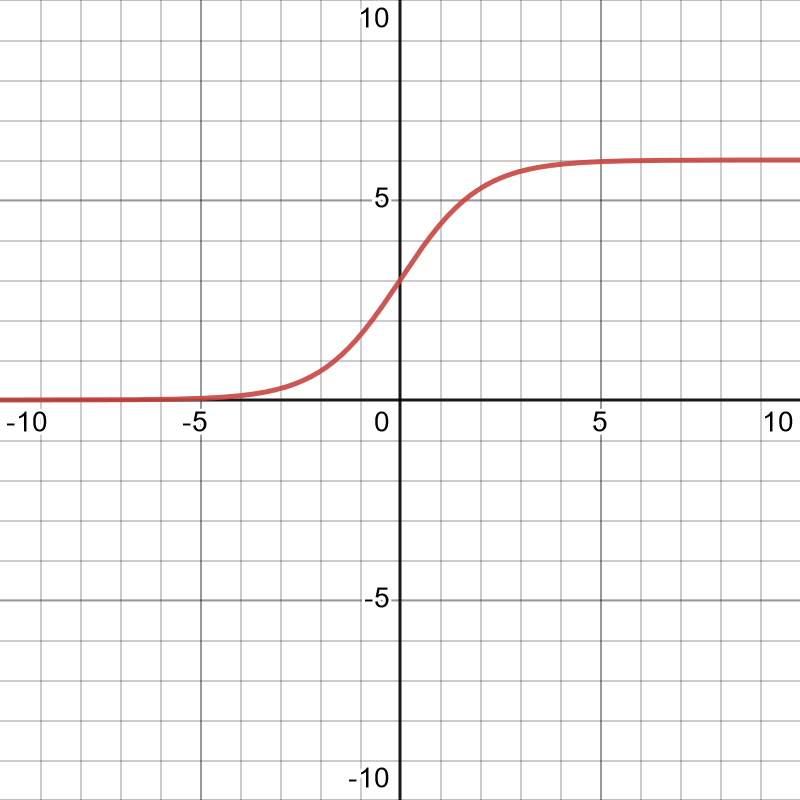
\includegraphics[scale=0.15]{desmos-graph(26).png}
\end{center}
From the picture, it's not entirely clear if $6$ is in the range. Maybe the graph of $y=Q(x)$ stays below the horizontal line
\mbox{$y=6$} or maybe it touches it, but the picture isn't decisive. To decide, you might try
numerical evaluation--say rounding to about 15 decimal places, we have
\begin{equation*}
    Q(45) = \frac{6}{1+\exp(-45)} = 6.00000000000000.
\end{equation*}
So you might conclude that indeed $6$ is in the range. But rounding to 42 decimal
places, the story is different:
\begin{equation*}
    Q(45) = \frac{6}{1+\exp(-45)} = 5.99999999999999999982824888516703638133671.
\end{equation*}
Now what do you think?

\quad To decide if $6$ is in the range, let's solve the equation:
\begin{align*}
    \left[ 6 = \frac{6}{1+\exp(-x)} \right] &= \left[1+\exp(-x) = 1 \right], 
                                            &\mbox{(cross multiply)}\\
                                            &= \left[\exp(-x) = 0 \right], 
                                            &\mbox{(subtract 1)}\\
                                            &= \varnothing  &\mbox{(zero not in range of $\exp$)}
\end{align*}
Since the solution set is empty, the number $6 \notin \range(Q)$.  Let's determine
if $0$ is in the range:
\begin{align*}
    \left[ 0 = \frac{6}{1+\exp(-x)} \right] &= \left[ 0 = 6 \right], 
                                            &\mbox{(cross multiply)}\\
                                            &= \varnothing  
\end{align*}
From the graph and the above calculations, almost surely we have \mbox{$\range(Q) = (0,6).$} 

\end{solution}

\newpage

\question[5] Define $Q(x) = (x-1)^2 + 1$ and $\dom(Q) = [1,\infty)$. Find the formula
and the domain of $Q^{-1}$. Use desmos to graph both $Q$ and $Q^{-1}$. As best you can,
reproduce your graphs here.
\begin{solution} First, let's find the formula for the  inverse function. We need to solve
\begin{align*}
 \left[ \left(y = (x-1)^2 + 1 \right) \right] &=  \left[ y -  1 = (x-1)^2\right],   & \mbox{(subtract 1)} \\
         &= \left[ \left(x-1 = -\sqrt{y -  1} \right) \lor  \left(x-1 = -\sqrt{y -  1} \right) \right],  \\
         &= \left[ \left(x = 1 -\sqrt{y -  1} \right) \lor  \left(x = 1 +\sqrt{y -  1} \right)\right]. & \mbox{(add 1)}
\end{align*}
Yikes! There are two solutions--that means the function isn't one-to-one. But wait! Remember the condition
\(1 \leq x\)?  The solution \(x = 1 -\sqrt{y -  1}\) gives a value for $x$ that is \emph{less} than one. So the
solution \(x = 1 -\sqrt{y -  1}\) is rubbish, leaving exactly one solution. 

\quad To find the domain of $Q^{-1}$ we need $1 + \sqrt{y -  1}$ to be real--that tells us that \mbox{$y \geq 1$}.  
Putting all together, we have $Q^{-1}(y) =  1 +  \sqrt{y -  1}$ and $\dom(Q^{-1}) = [1,\infty)$.
Here are my graphs:

\begin{center}
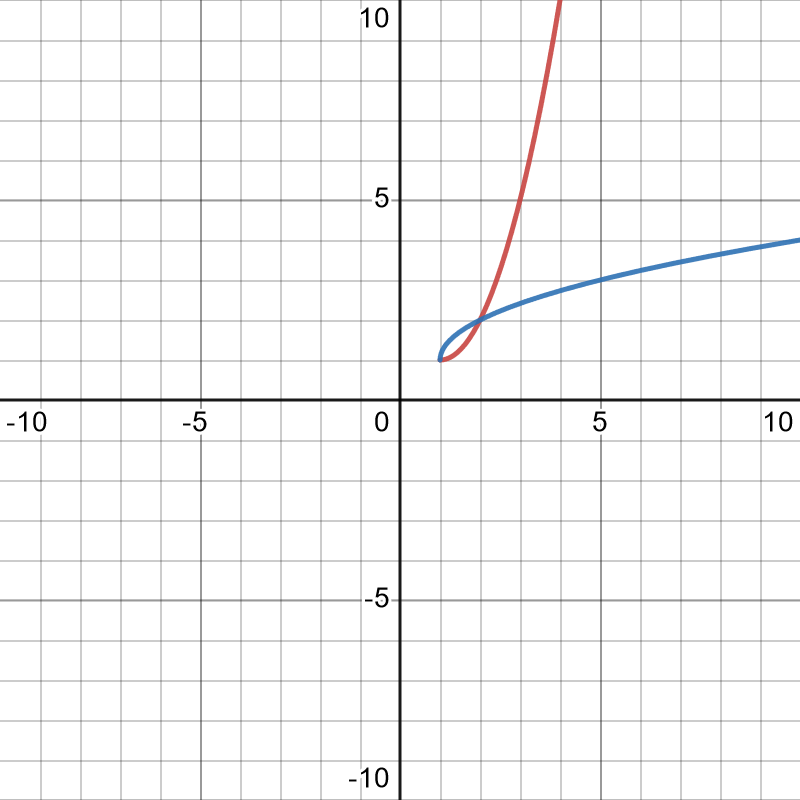
\includegraphics[scale=0.25]{desmos-graph(27).png}
\end{center}


\end{solution}
\end{questions}
\end{document}